\begin{frame}{Finite Element Analysis}
\begin{columns}
\column{0.58\linewidth}
\centering
\begin{outline}
  \1 Numerically solve differential equations
  \2 Geometric domains
  \2 Boundary Conditions
  \1 Example uses:
  \2 Linear elasticity
  \2 Thermal transfer
  \2 Fluid flow
  \1 Aid in design, testing, and validation
\end{outline}

\column{0.38\linewidth}
\begin{center}
\begin{align*}
  \sigma + F &= 0\\
             &\\
  \nabla t &= 0
\end{align*}

\shadowimage[width=4cm]{wiki_car_example.png} 

\end{center}
\end{columns}
\blfootnote{Image from \href{https://en.wikipedia.org/wiki/Finite_element_method}{Wikipedia}}
\end{frame}

\begin{frame}{Bracket Example}
  \centering
  \begin{center}
    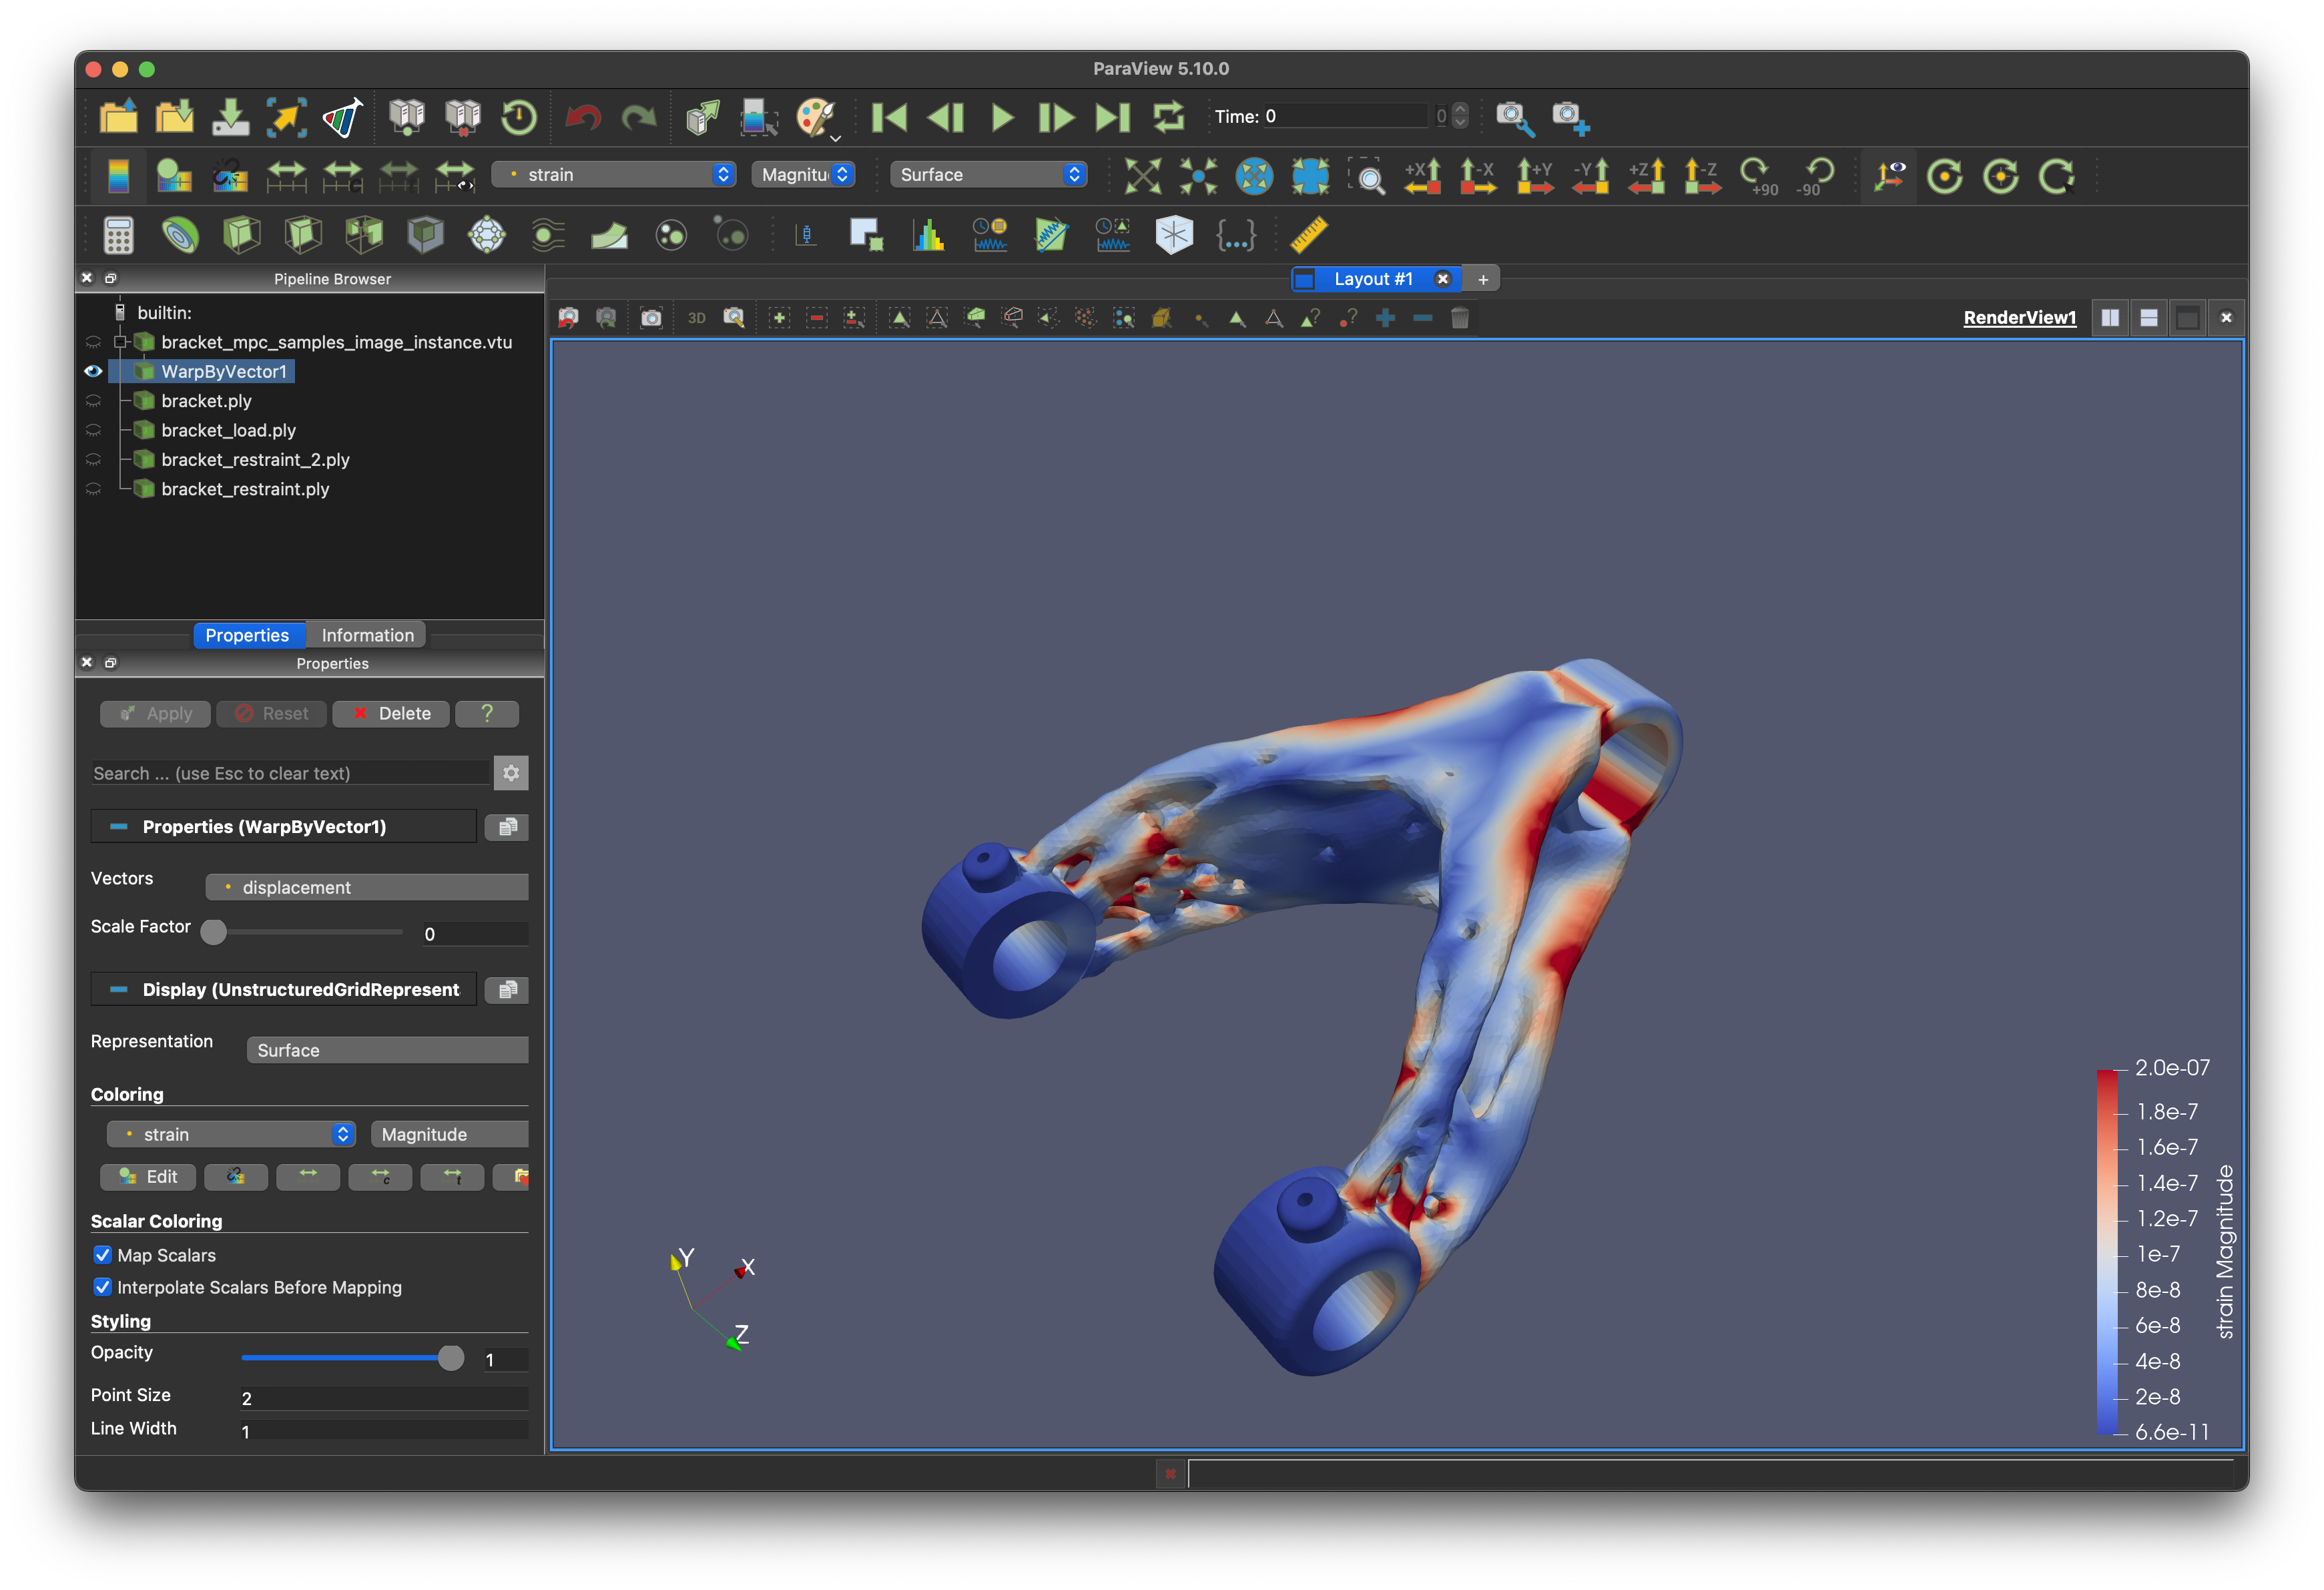
\includegraphics[width=0.7\linewidth]{bracket_demo.png}
  \end{center}
\end{frame}


